% Created 2014-11-08 Sat 11:30
\documentclass[presentation, bigger]{beamer}
\usepackage[utf8]{inputenc}
\usepackage[T1]{fontenc}
\usepackage{fixltx2e}
\usepackage{graphicx}
\usepackage{longtable}
\usepackage{float}
\usepackage{wrapfig}
\usepackage[normalem]{ulem}
\usepackage{textcomp}
\usepackage{marvosym}
\usepackage{wasysym}
\usepackage{latexsym}
\usepackage{amssymb}
\usepackage{amstext}
\usepackage{hyperref}
\usepackage{url}
\usepackage{multimedia}
\usepackage[dutch]{babel}
\usepackage[font=scriptsize,labelfont=bf]{caption}
\setbeamertemplate{caption}[numbered]
\usepackage{pgfpages}
\setbeameroption{show notes on second screen=right}

\tolerance=1000
\usetheme{kuleuven}
\useinnertheme{rectangles}
\graphicspath{{graphics/}}
\usepackage[style=authoryear,hyperref,backref,square,natbib,ibidtracker=false]{biblatex}
\bibliography{bibliography}

\usepackage{graphicx}
\usetheme{default}
\author{Ward Schodts, Xavier Goás Aguililla}
\date{maandag 10 november 2014}
\title{Internet of Things code deployment metrics}
\hypersetup{
  pdfkeywords={},
  pdfsubject={},
  pdfcreator={Emacs 24.3.1 (Org mode N/A)}}



\newcommand{\aheader}[2]{\action<#1-|alert@#1>{#2}}
% first argument: slide number to appear from, second argument: content of header 
\newcommand{\hiddencell}[2]{\action<#1->{#2}}
% first argument: slide number to appear from, second argument: content of cell

\DeclareBibliographyCategory{papers}


\begin{document}

\maketitle
\begin{frame}[noframenumbering]{Outline}
  \tableofcontents
  \note{3 grote luiken\\
        }
\end{frame}



\section{Inleiding tot wireless sensor networks}
\label{sec-1}
\begin{frame}[label=sec-1-1]{Wireless sensor networks: wat zijn ze? (1)}

  \begin{figure}
    \fbox{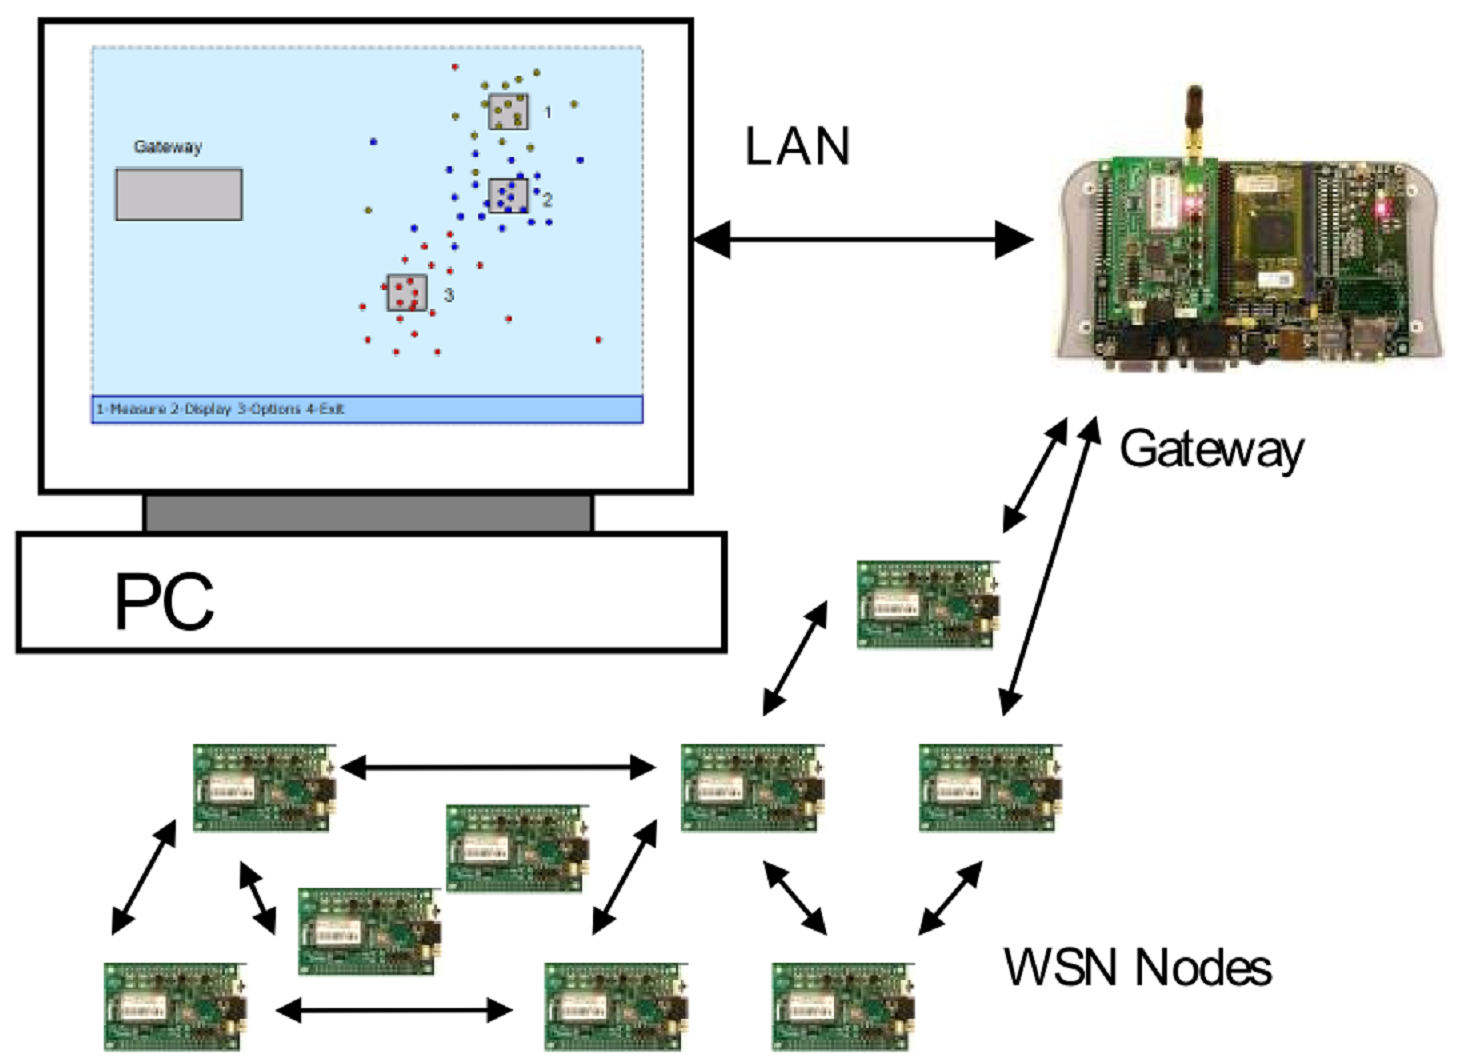
\includegraphics[width=0.82\textwidth,keepaspectration=true]{intro/overview.png}}
    \caption{Een wireless sensor network}
  \end{figure}
  \note{
\begin{itemize}
\item heel veel, sensoren enkele gateways
\item netwerk bestaande uit sensoren
\item ad-hoc netwerk technieken, geen bestaande!
\item geen routing door 1 centrale unit
\item communiceren via elkaar

\end{itemize}
}
\end{frame}

\begin{frame}[label=sec-1-2]{Wireless sensor networks: wat zijn ze? (2)}
  \begin{figure}
    \fbox{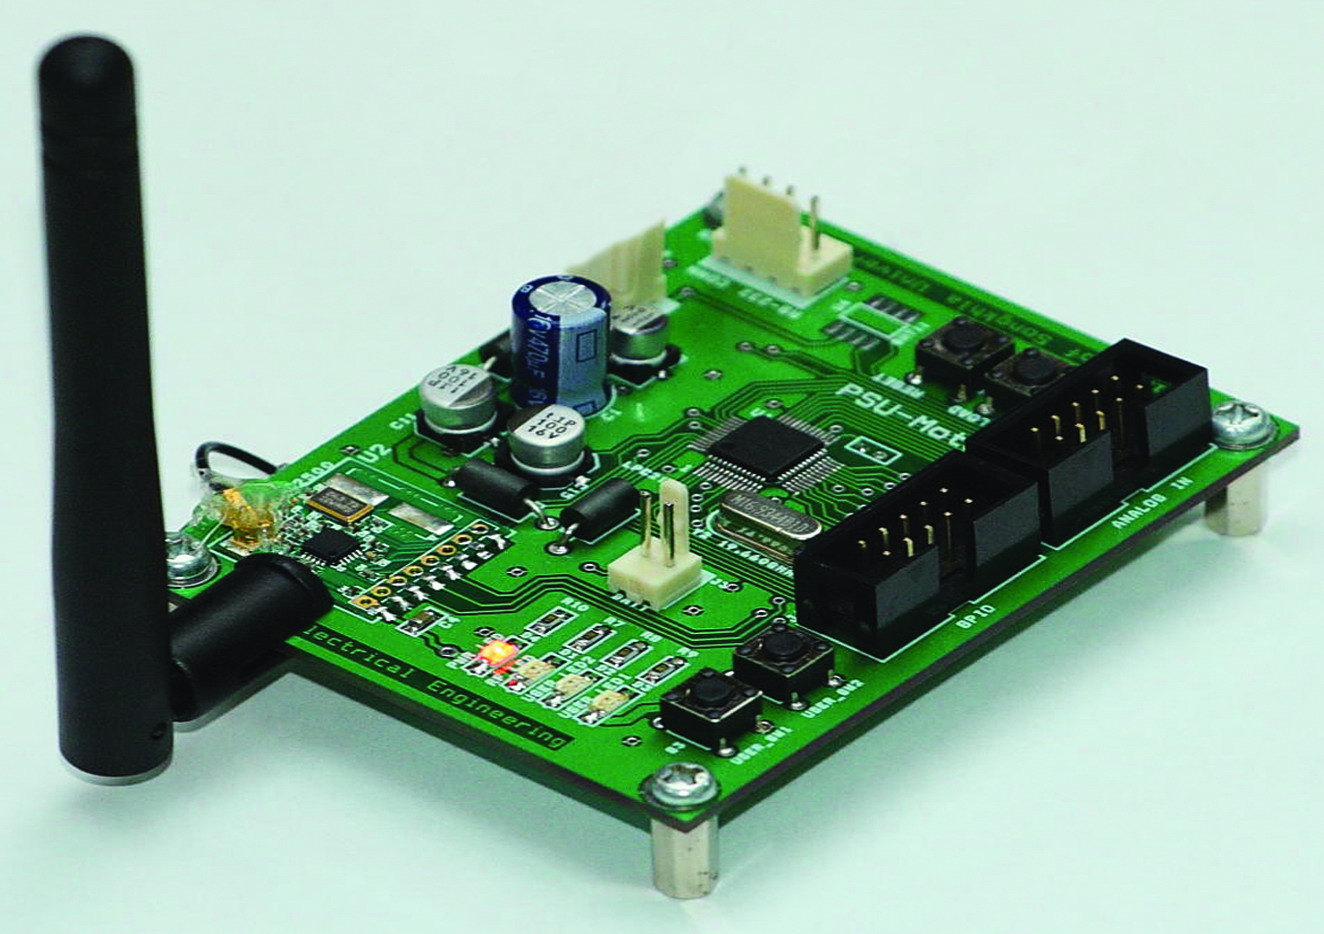
\includegraphics[height=0.78\textheight,keepaspectration=true]{intro/psumote.jpg}}
    \caption{Een PSUMote}
  \end{figure}
\note{
\begin{itemize}
\item embedded device
\item RF antenne, geen wifi, minder energie, groter bereik
\item sensoren worden aangesloten
\item microcontroller COMPUTEr ON A CHIP
\end{itemize}
}
\end{frame}



\begin{frame}[label=sec-1-3]{Toepassingen van WSN}
  \centering 
  \begin{tabular}{c c c}
    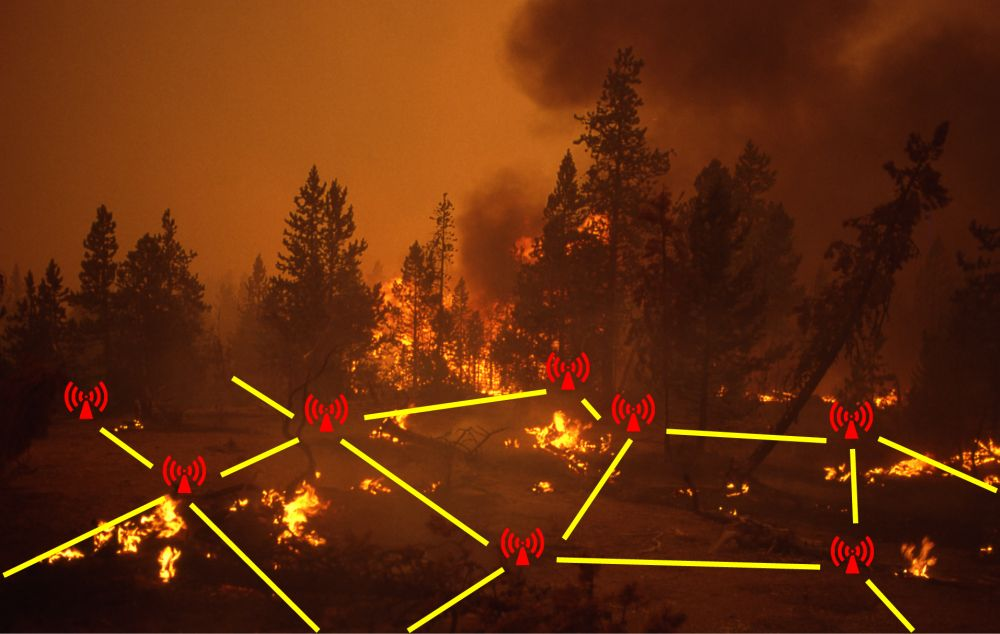
\includegraphics[width=5.25cm,keepaspectration=true]{graphics/sample_applications/fire.jpg}
    & 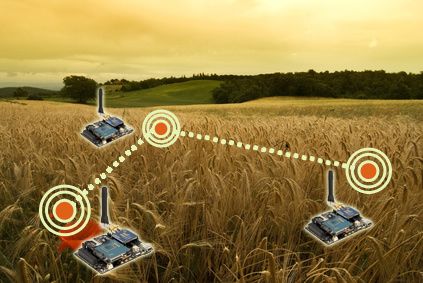
\includegraphics[width=5cm,keepaspectration=true]{graphics/sample_applications/landbouw.jpg} \\
    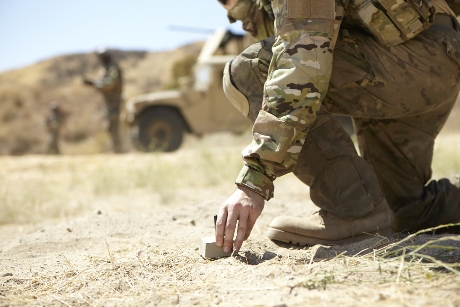
\includegraphics[width=5.25cm,keepaspectration=true]{graphics/sample_applications/military.jpg}
    & 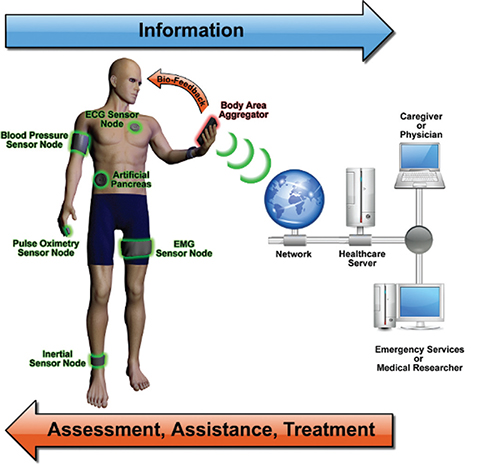
\includegraphics[width=5cm,keepaspectration=true]{graphics/sample_applications/medicine.jpg}
  \end{tabular}
  \note{
  \begin{itemize}
  \item bosbranden
  \item landbouw
  \item militaire doeleinden
  \item geneeskunde
  \end{itemize}
}
\end{frame}

\begin{frame}[label=sec-1-4]{Great Duck Island experiment I}
  \centering
  \begin{figure}
    \fbox{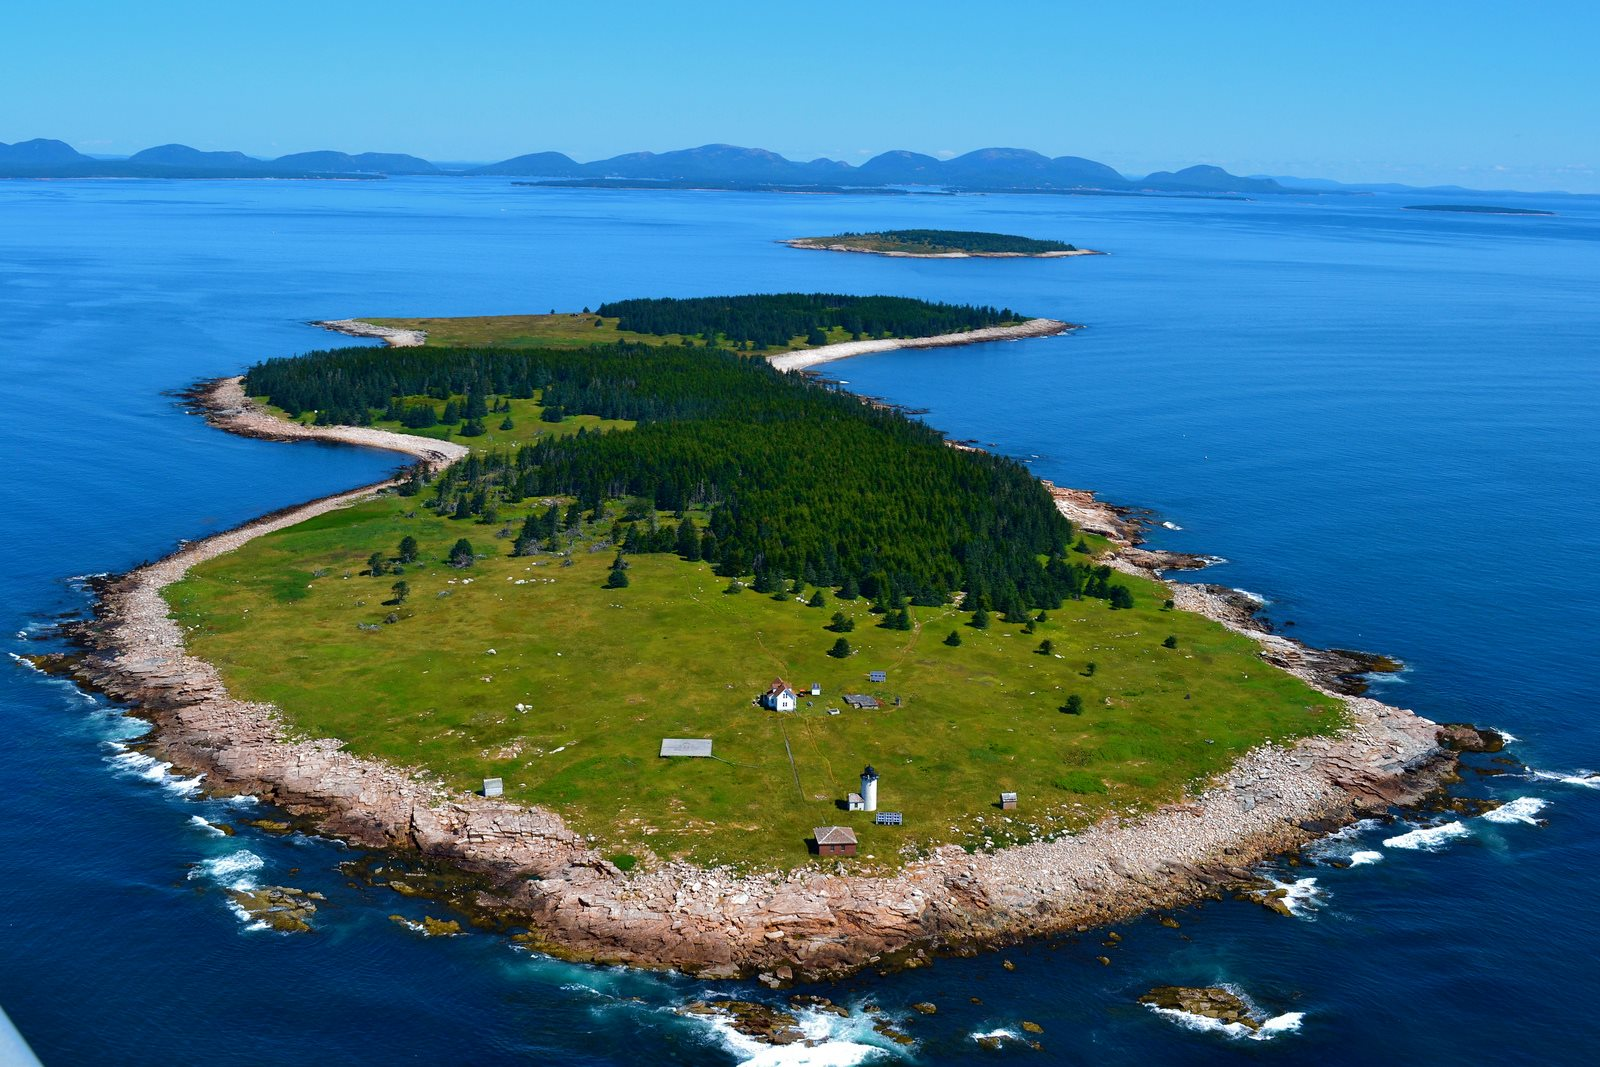
\includegraphics[width=0.85\textwidth,keepaspectratio=true]{gdi/gdi.jpg}}
    \caption{Great Duck Island}
  \end{figure}
 \note{
 \begin{itemize}
 \item experiment uit paper
 \item biologen wouden vogels bestuderen
 
\end{itemize}  }
 
\end{frame}
% TODO Beter woord voor monitoring vinden
\begin{frame}[label=sec-1-5]{Great Duck Island experiment II}
  \begin{figure}
    \begin{minipage}{.5\textwidth}
      \centering
      \fbox{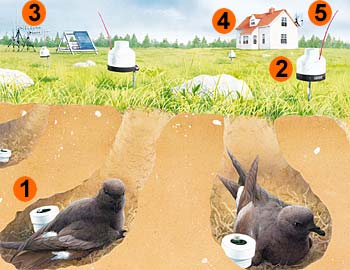
\includegraphics[width=.8\textwidth]{gdi/gdi_duckmote.jpg}} 
      \captionof{figure}{Motes in nesten}
    \end{minipage}%
    \begin{minipage}{.5\textwidth}
      \centering
      \fbox{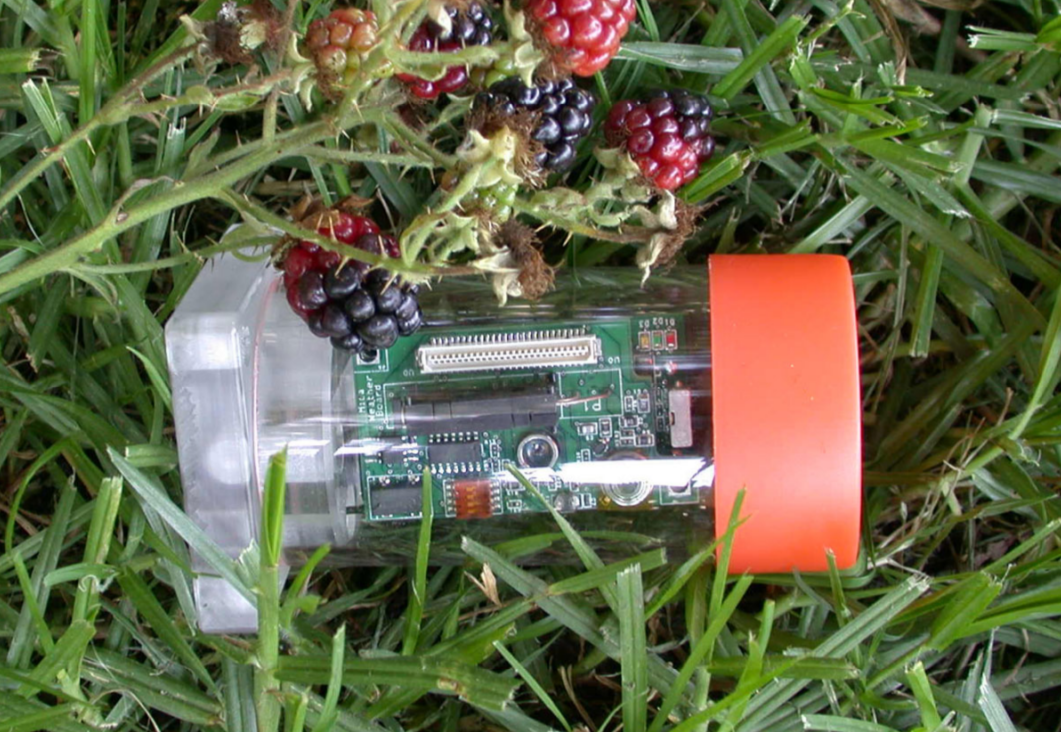
\includegraphics[width=.8\textwidth]{gdi/micamote.png}}
      \captionof{figure}{Motes in het gras}
    \end{minipage}
  \end{figure}
  \begin{itemize}
  \item habitat monitoring van vogels
  \item motes in broedholen
  \item 7 maanden
  \end{itemize}
  \note{
  \begin{itemize}
    \item Mensen konden niet in de buurt komen zonder te storen
    \item In de holen werden de motes gelegd
    \item En aanvullingen werden bijgezet
  \end{itemize}

  }
 
\end{frame}

\begin{frame}[label=sec-1-6]{Belangrijke aspecten bij WSN-design}
  \uncover<2->{\begin{block}{energie-effici\"ent}
      tot 10 jaar meegaan op \'e\'en batterij
    \end{block}}%
  \uncover<3->{\begin{block}{dichtheid}
      tot 20 sensor nodes per $m^3$ (geen harde limiet)
    \end{block}}%
  \uncover<4->{\begin{block}{goedkoop}
      \$1 of minder voor heel grootschalige deployments
    \end{block}}%
  \uncover<5->{\begin{block}{autonoom}
      deploy and forget
    \end{block}}%
  \uncover<6->{\begin{block}{adaptief}
      makkelijke aanpasbare topologie, bestand tegen falen van motes
    \end{block}}
  \note{
  \begin{itemize}
  \item energie efficeit tot 10 jaar
  \item dichtheid, zie geneeskunde
  \item grote hoeveelheid, dus moet goedkoop, moet kapot gaan
  \item autonoom deploy and forget
  \item adaptief, topologie verandert, falende motes
  \end{itemize}}
\end{frame}

\section{Middleware voor WSNs}
\label{sec-2}
\begin{frame}[label=sec-2-1]{Wat is middleware?}
  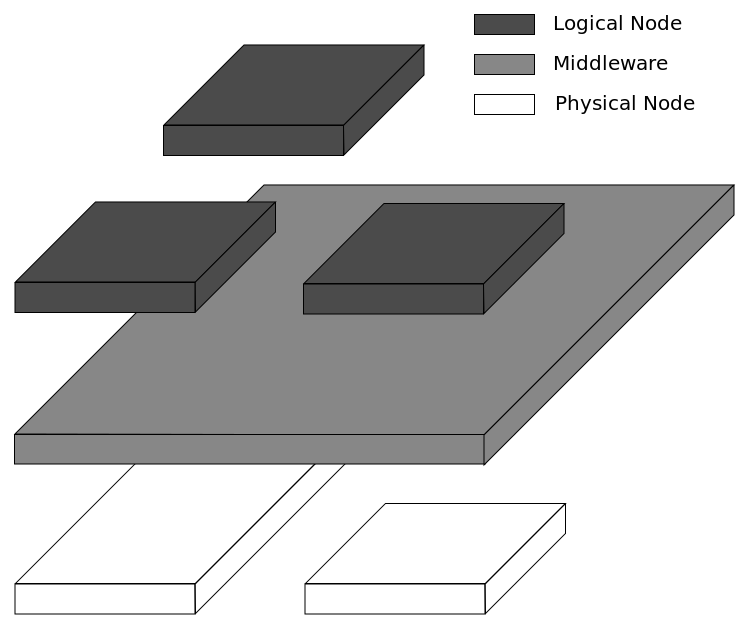
\includegraphics[width=0.9\textwidth, height=0.8\textheight,keepaspectration=false]{looci/schema.png}
\note{\begin{itemize}
\item uitgebreide verz architeturen in WSN $\rightarrow$ physical node
\item gedistriubeerde systeem is hetrogeen
\item verschillende ossen
\item laag tussen os en applicatie die funcitonaliteit aanbied
\item middleware zorgt voor consitente manier van programmeren
\end{itemize}



}
\end{frame}

\begin{frame}[label=sec-2-2]{Mogelijke aanpakken}

\begin{minipage}{.5\textwidth}
{\large Zonder middleware}
\begin{itemize}
\item Monolithische aanpak; bv. TinyOS
\end{itemize}
{\large Met middleware}
\begin{itemize}
  \item application-based; bv. Contiki, Squawk
  \item component-based; bv. OpenCOM, Figaro, LooCi
  \end{itemize}
      
    \end{minipage}%
\begin{minipage}{.5\textwidth}
      \centering
      \fbox{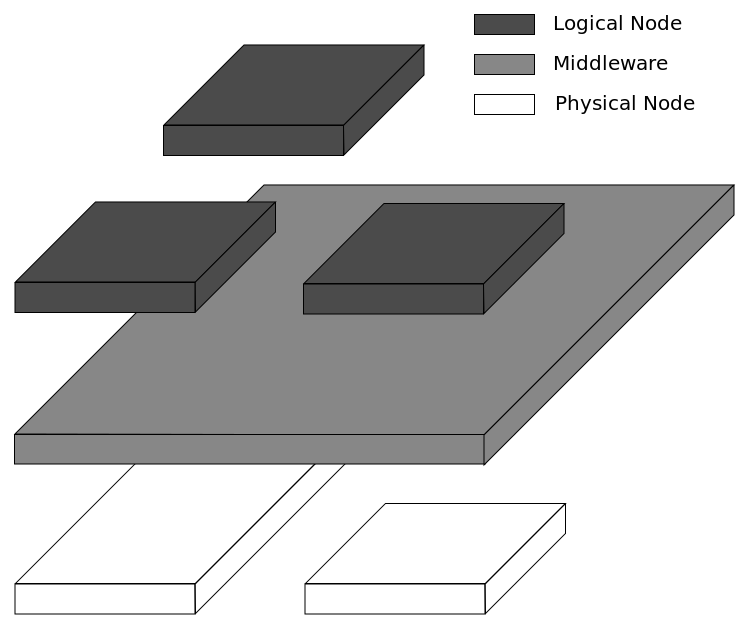
\includegraphics[width=.8\textwidth]{looci/schema.png}} 
      
    \end{minipage}


\note{
\begin{itemize}
\item granularity
\item Monolithisch = OS + app\\
\item applicationbased = os en apps gescheiden
\item component-based = at runtime component in app

\end{itemize}
}


\end{frame}

\begin{frame}[label=sec-2-3]{LooCi (1)}
  \begin{columns}[t]
    \column{.5\textwidth}
    \centering
    
\includegraphics[width=5cm,keepaspectration=true]{looci/looci.png}\\
    
\includegraphics[width=5cm,keepaspectration=true]{looci/distrinet.png}
    \column{.5\textwidth}
    \centering
    \begin{itemize}
    \item Ontwikkeld aan KULeuven
    \item Runtime deployable components
    \item Werkt op Contiki, Sun SPOT, OSGi en Android
    \end{itemize}
  \end{columns}
  \note{\begin{itemize}
    \item Ontwikkeld aan KULeuven
    \item Runtime deployable components
    \item Werkt op Contiki, Sun SPOT, OSGi en Android
    \end{itemize}}
\end{frame}

\begin{frame}[label=sec-2-4]{LooCi (2)}
  \centering
  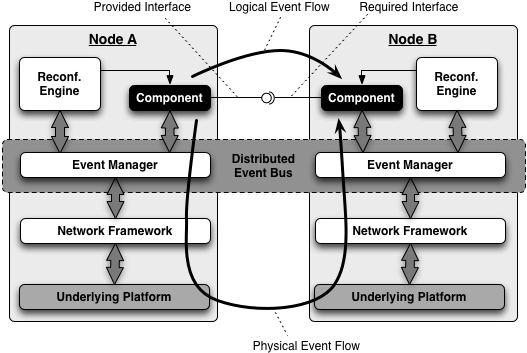
\includegraphics[width=0.9\textwidth,keepaspectration=true]{looci/LooCIExecEnvironment.png}
\note{It provides a clean separation of distribution concerns from component implementation}
\end{frame}

\begin{frame}[label=sec-2-5]{LooCi demo}
  
\end{frame}

\section{Energieverbruik}
\label{sec-3}

\begin{frame}[label=sec-1-7]{Store, compute, transmit?}
  \begin{itemize}
  \item drie grote factoren in energieverbruik:
    \vfill
    \begin{tabular}{c c c}
      \hiddencell{2}{
\includegraphics[width=0.25\textwidth,keepaspectration=true]{storage}} & \hiddencell{3}{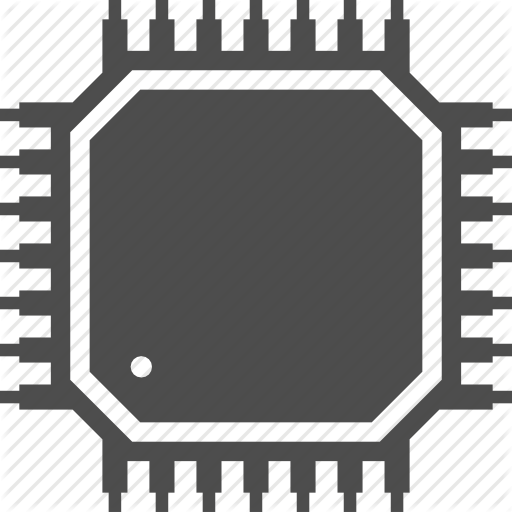
\includegraphics[width=0.25\textwidth,keepaspectration=true]{cpu}} & \hiddencell{4}{
\includegraphics[width=0.25\textwidth,keepaspectration=true]{radio}}  \\
      \hiddencell{2}{flash-opslag} & \hiddencell{3}{berekeningen} & \hiddencell{4}{netwerkoverdracht}
    \end{tabular}
    \vfill
  \item ook sensoren aangesloten op microcontroller hebben invloed
  \end{itemize}

    \note{
      \begin{itemize}
      \item antennes op en aan zetten kost veel energie
      \item flash en CPU iets minder, maar:
        \begin{itemize}
        \item lage kloksnelheid 
          \begin{itemize}
          \item slechte concurrency, 
          \item slechte performantie in het algemeen
          \end{itemize}
        \item beperkte hoeveelheid geheugen
        \end{itemize}
      \item huidige aanpak: veel netwerkoverdracht, weinig CPU- en geheugengebruik
      \item waarom voor sommige dingen geen CPU en flash gebruiken? bv. temperatuurmetingen
      \item doel: kijken hoe doenbaar dit is
      \end{itemize}
    }

\end{frame}


\begin{frame}[label=sec-3-2]{Hoe meten we het?}
  \begin{minipage}{\textwidth}
    \centering
    \fbox{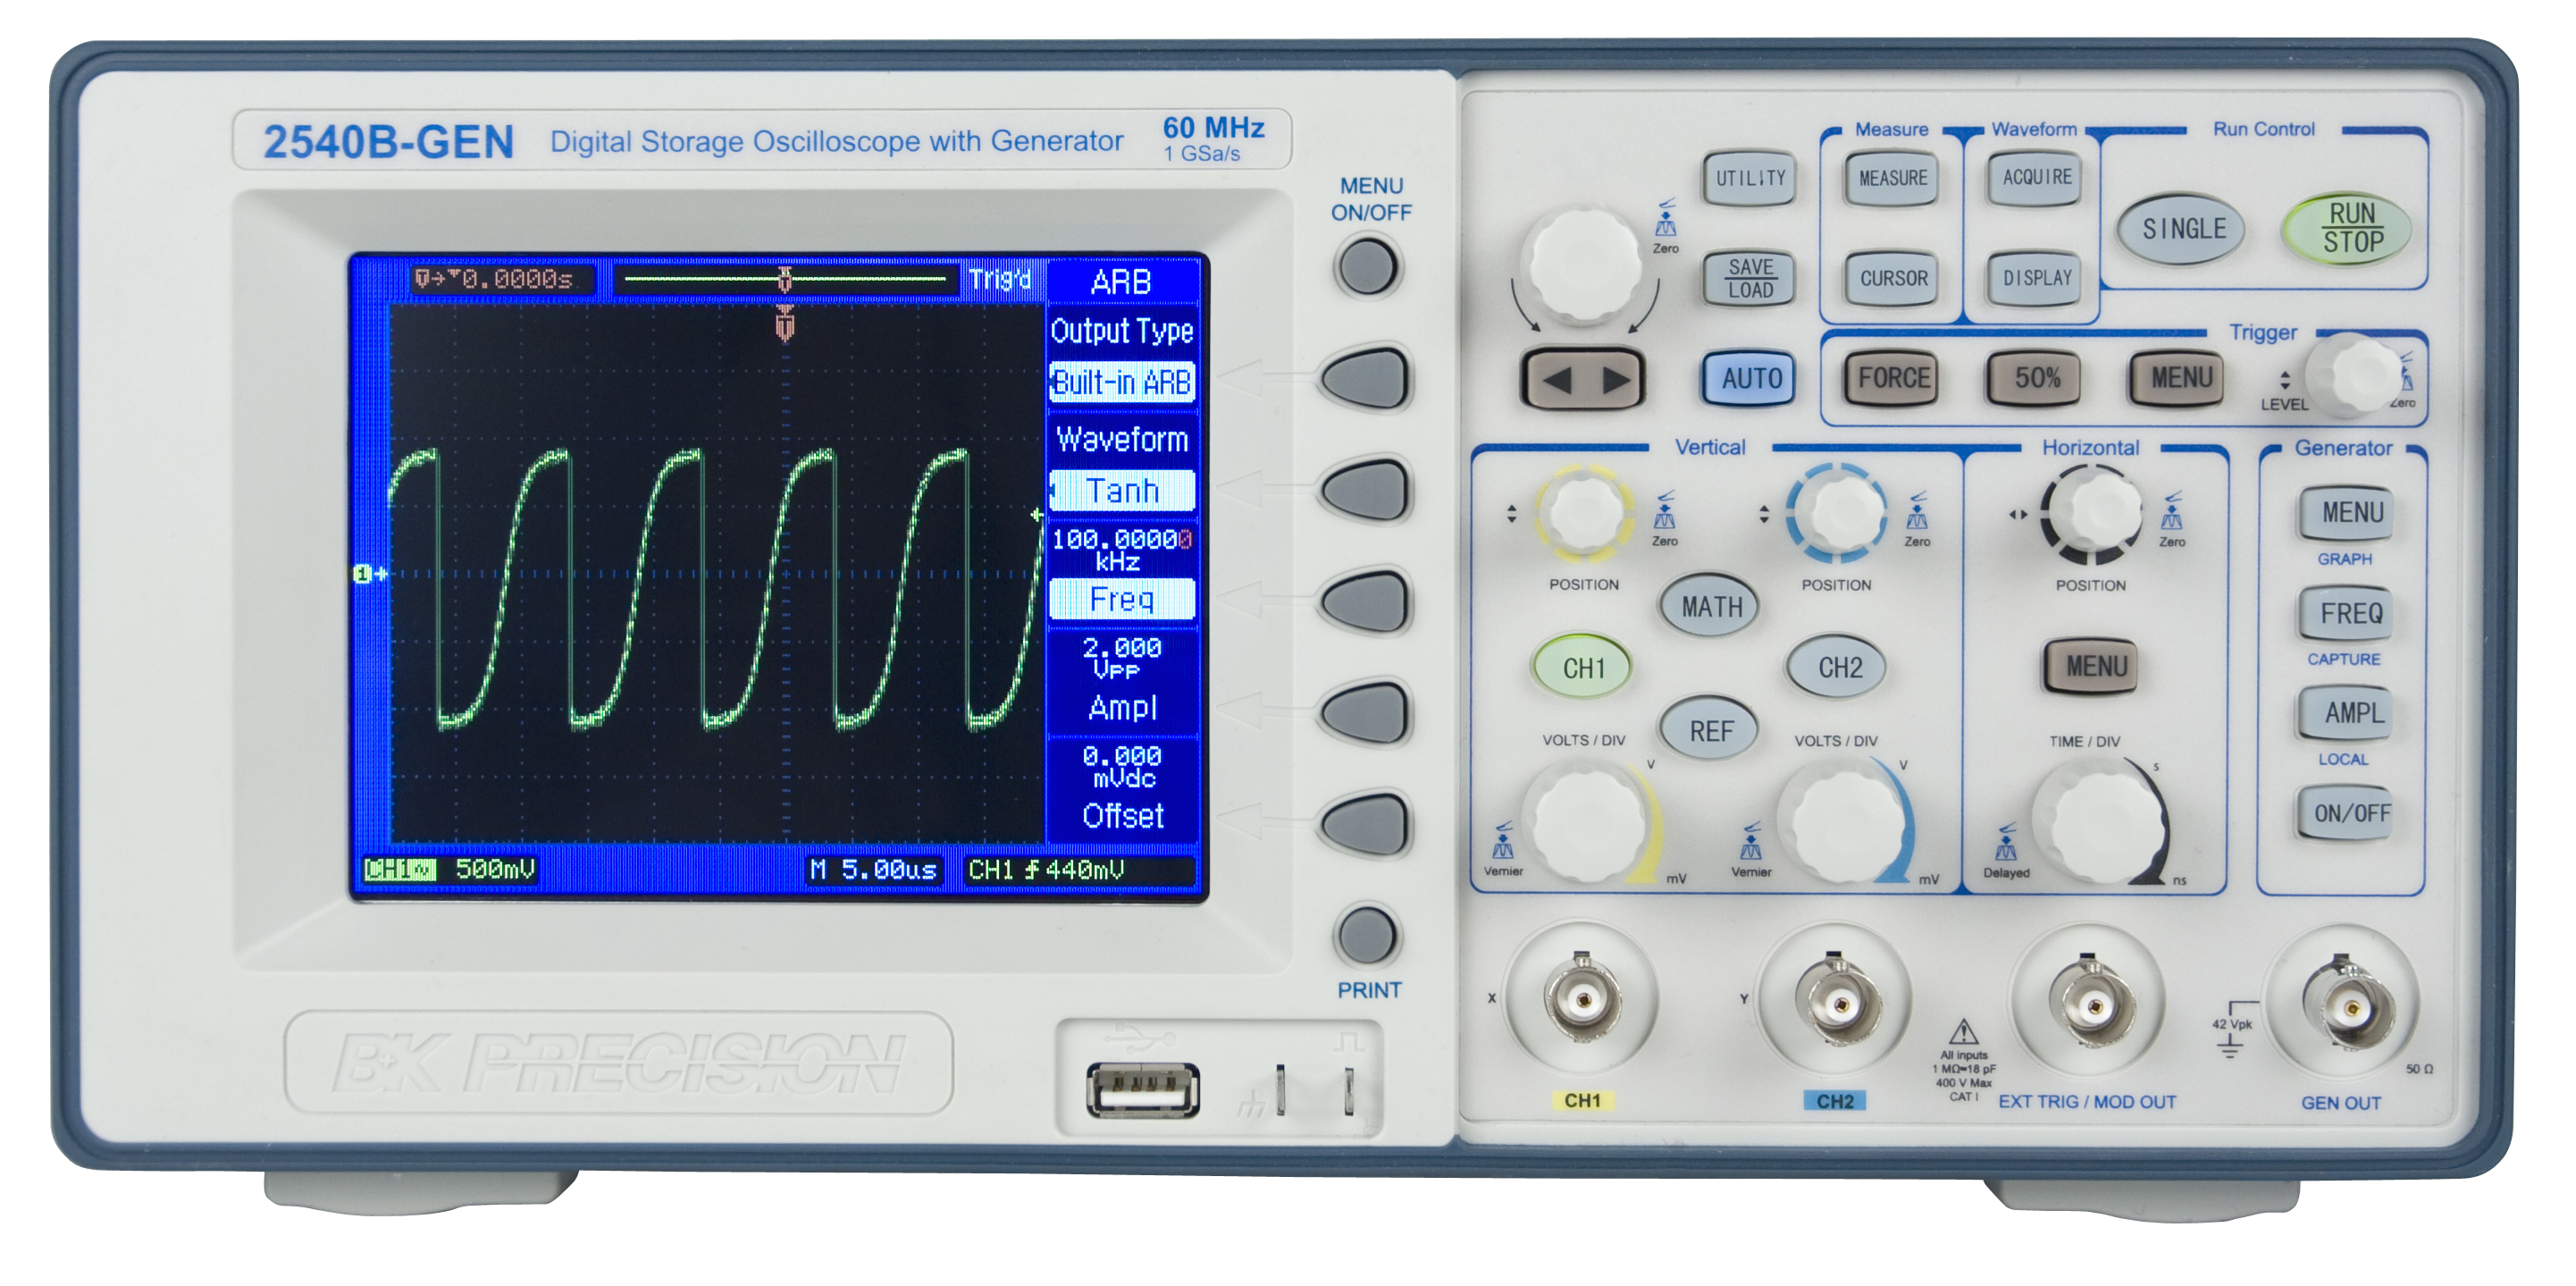
\includegraphics[width=0.9\textwidth,keepaspectration=true]{elek/dso.jpg}} 
    \captionof{figure}{Oscilloscoop}
  \end{minipage}

  \note{
    \begin{itemize}
    \item oscilloscopes are used to observe the change of an electrical signal over time
    \item voltage and time describe a shape which is continuously graphed against a calibrated scale
    \item observed waveform can be analyzed for such properties 
      \begin{itemize}
      \item amplitude
      \item frequency
      \item rise time
      \item time interval
      \item distortion 
      \item etc.
      \end{itemize}
    \end{itemize}
    
  }
\end{frame}

\begin{frame}[label=sec-3-3]{Meetopstelling}
  \begin{figure}[center]
    \centering
    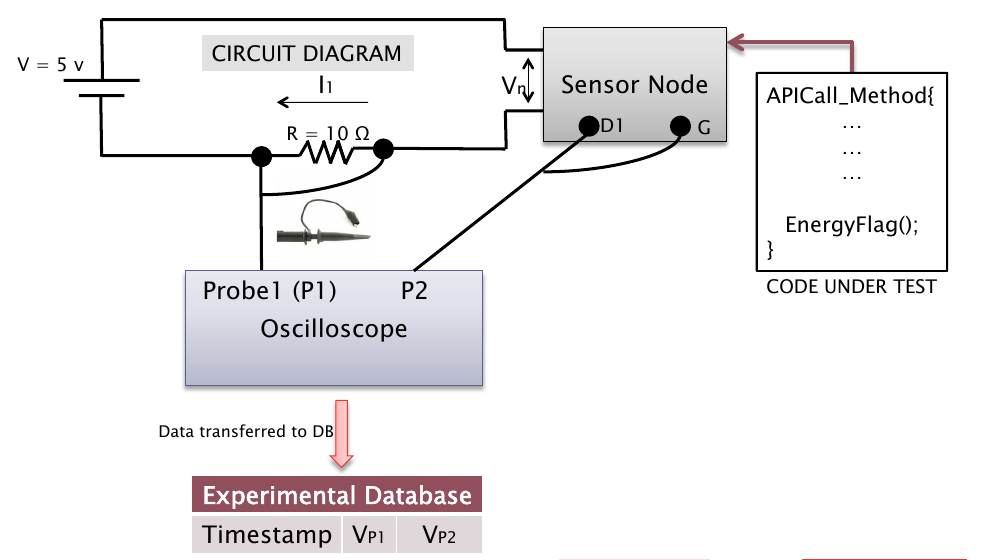
\includegraphics[width=0.9\textwidth,keepaspectration=true]{elek/diag1}
    \caption{Meetopstelling}
  \end{figure}
  \note{

    \begin{itemize}
    \item stroomverbruik van bepaalde methodes plotten
    \item opstelling: weerstand in serie geplaatst met stroomtoevoer
    \item oscilloscoop meet spanning
    \item start en stop mbv output pin
    \item outputpin softwarematig getriggerd
    \end{itemize}

Meetmethode:\\
\begin{itemize}
\item meerdere keren het te meten stuk code oproepen
\item pin zal verscheidene keren aan en uit flippen en metingen triggeren
\end{itemize}
  }
\end{frame}

\begin{frame}[label=sec-3-4]{Voltageplot}
  \begin{figure}
    \centering
    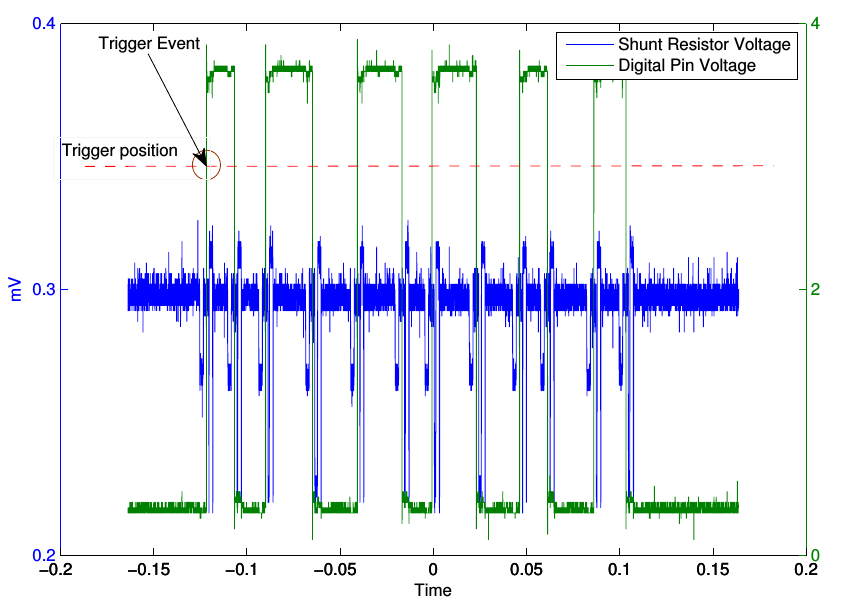
\includegraphics[width=0.85\textwidth,keepaspectration=true]{elek/energy_measurement_plot.png}
    \caption{Voltageplot}
  \end{figure}
  \note{
    Ziet er als volgt uit.

    \begin{itemize}
    \item blauw: voltage over weerstand
    \item groen: voltage op pin
    \item kan veel uit afgeleid worden!
    \end{itemize}
  }
\end{frame}

\begin{frame}[label=sec-3-5]{Analyse energieverbruik}
  \begin{itemize}
  \item wet van Ohm!
    \begin{figure}
      \centering
      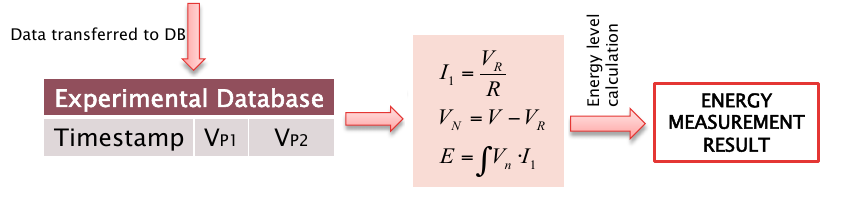
\includegraphics[width=0.9\textwidth,keepaspectration=true]{elek/diag2}

      \caption{Stroomverbruikanalyse}
    \end{figure}
  \item modelleren m.b.v. lineaire regressie
  \end{itemize}
  \note{

    \begin{itemize}
    \item gebruik de wet van Ohm
    \item accurate metingen van stroomverbruik van bepaalde methodes
    \item herhaal metingen tot we een goed idee hebben van \\ gemiddeld verbruik
    \end{itemize}

  }
\end{frame}
\section{Conclusie}
\label{sec-4}
\begin{frame}[label=sec-4-1]{Waar komen wij in het spel?}
  \begin{itemize}
  \item huidige aanpak in het veld: netwerk-overdracht
  \item is dit wel de enige goede methode?
  \item analyse stroomverbruik voor verschillende types code deployment
  \item implementeren tool voor simulatie energieverbruik
  \end{itemize}
  \note{

    \begin{itemize}
    \item paper gebruikt het voor meten van kost van reconfiguratie
    \item wij gaan het toepassen op code deployment
    \item d.w.z. is het interessanter om deze methode te \\ draaien op sensor node of op server?
    \end{itemize}

  }
\end{frame}

\begin{frame}[label=sec-4-2]{Conclusie}
  \begin{itemize}
  \item momenteel weinig aandacht voor alternatieve code deployment
  \item we hebben jullie een aantal idee\"en getoond 
  \item hier gaan we iets aan doen!
  \end{itemize}
\end{frame}
\begin{frame}[allowframebreaks]{Bibliografie}

\addtocategory{papers}{akyildiz2002wireless}
\addtocategory{papers}{mainwaring2002wireless}
\addtocategory{papers}{hughes2009looci}
\addtocategory{papers}{hughes2013energy}
  \nocite{*}
  \textbf{Papers}
  \printbibliography[category=papers]
  \newpage
  \textbf{Afbeeldingen}
  \printbibliography[type=misc]
\end{frame}

% Emacs 24.3.1 (Org mode N/A)
\end{document}
